\documentclass{article}
\usepackage[a3paper,landscape,margin=8mm]{geometry}
\usepackage{tikz}
\usepackage{fontspec}
\setmainfont{Inter}
\pagestyle{empty}

\begin{document}

%% ============================================================
%% PAGE 1: 435 x 70mm blank wireframe (92% scale)
%% ============================================================

\noindent
\begin{center}
{\fontsize{13}{16}\selectfont\bfseries TheStreamDeck -- Blank Wireframe (70mm)}\\[1pt]
{\fontsize{8}{10}\selectfont\color{gray} 92\% scale on A3 (actual: 435 x 70mm). Clean real estate for free sketching.}
\end{center}
\vspace{8mm}

\begin{center}
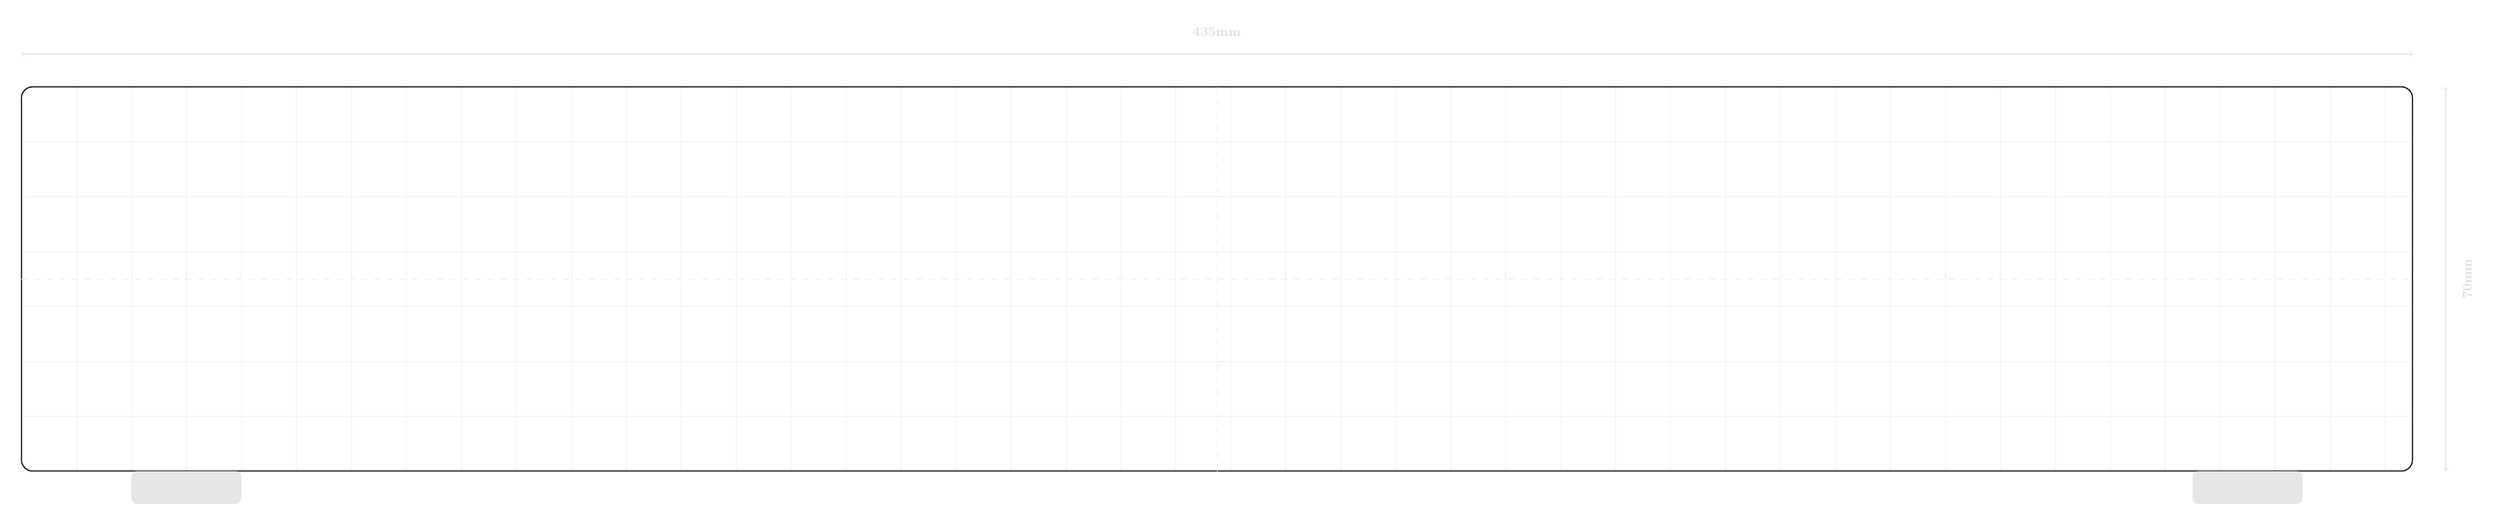
\begin{tikzpicture}[x=0.92mm, y=0.92mm]
  \def\cw{435} \def\ch{70}

  % Light grid (10mm)
  \begin{scope}
    \clip[rounded corners=1.8mm] (0,0) rectangle (\cw,\ch);
    \foreach \x in {0,10,...,435} { \draw[gray!12, line width=0.15pt] (\x,0) -- (\x,\ch); }
    \foreach \y in {0,10,...,70} { \draw[gray!12, line width=0.15pt] (0,\y) -- (\cw,\y); }
  \end{scope}

  % Case outline
  \draw[black, line width=0.5pt, rounded corners=1.8mm] (0,0) rectangle (\cw,\ch);

  % Centre crosshair (very subtle)
  \draw[gray!15, line width=0.3pt, dashed] (\cw/2,0) -- (\cw/2,\ch);
  \draw[gray!15, line width=0.3pt, dashed] (0,\ch/2) -- (\cw,\ch/2);

  % Feet
  \fill[gray!20, rounded corners=1mm] (20,-6) rectangle (40,0);
  \fill[gray!20, rounded corners=1mm] (\cw-40,-6) rectangle (\cw-20,0);

  % Dimensions
  \draw[gray!30, line width=0.2pt, <->] (0,\ch+6) -- (\cw,\ch+6);
  \node[font=\fontsize{6}{8}\selectfont, text=gray!35] at (\cw/2,\ch+10) {435mm};
  \draw[gray!30, line width=0.2pt, <->] (\cw+6,0) -- (\cw+6,\ch);
  \node[font=\fontsize{6}{8}\selectfont, text=gray!35, rotate=90] at (\cw+10,\ch/2) {70mm};
\end{tikzpicture}
\end{center}

\vspace{12mm}

% Second copy for another sketch
\begin{center}
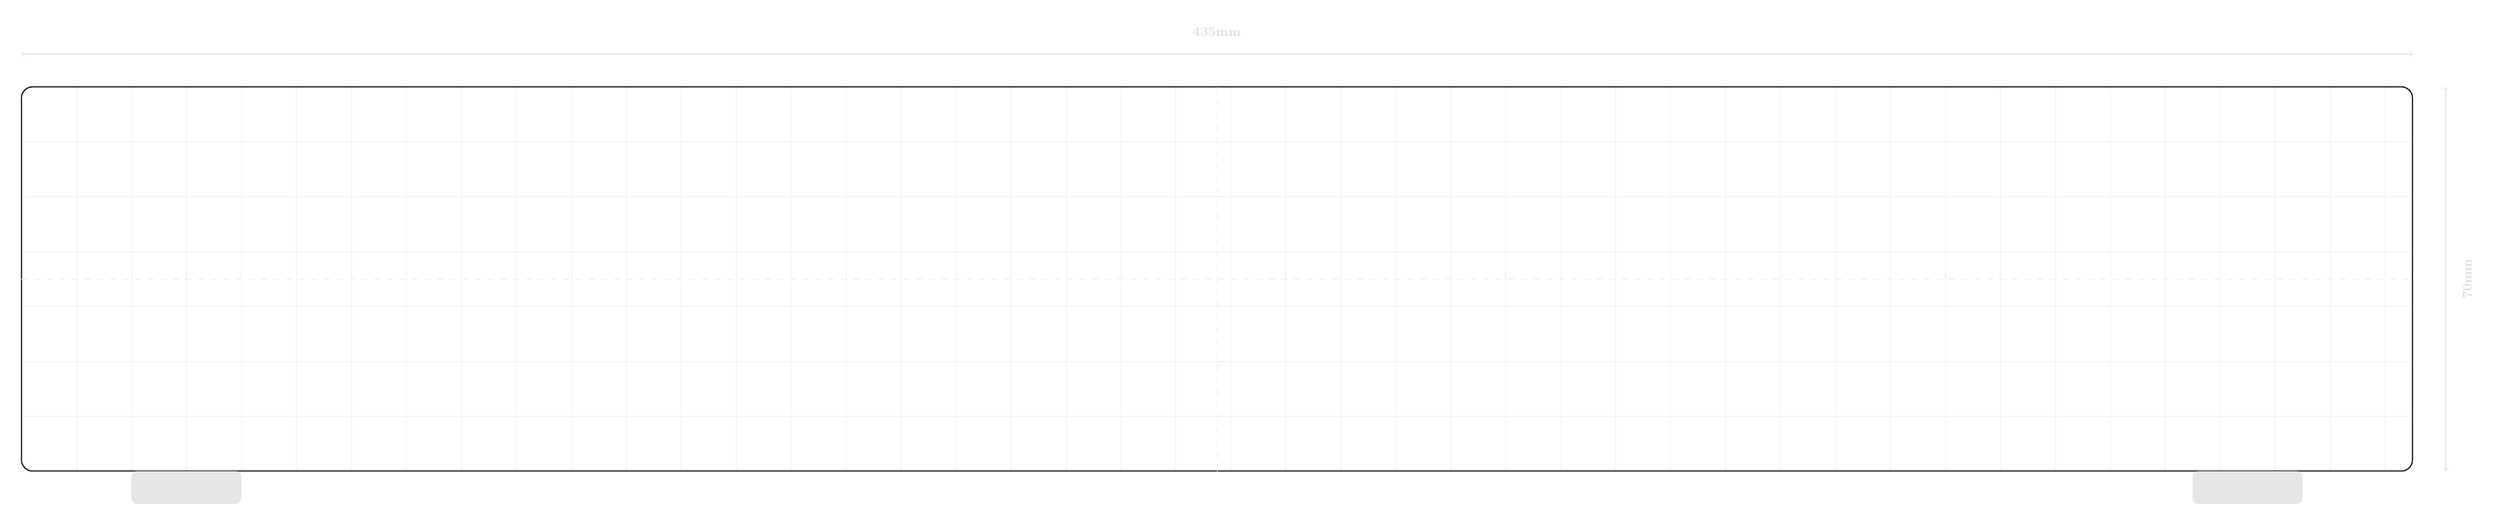
\begin{tikzpicture}[x=0.92mm, y=0.92mm]
  \def\cw{435} \def\ch{70}
  \begin{scope}
    \clip[rounded corners=1.8mm] (0,0) rectangle (\cw,\ch);
    \foreach \x in {0,10,...,435} { \draw[gray!12, line width=0.15pt] (\x,0) -- (\x,\ch); }
    \foreach \y in {0,10,...,70} { \draw[gray!12, line width=0.15pt] (0,\y) -- (\cw,\y); }
  \end{scope}
  \draw[black, line width=0.5pt, rounded corners=1.8mm] (0,0) rectangle (\cw,\ch);
  \draw[gray!15, line width=0.3pt, dashed] (\cw/2,0) -- (\cw/2,\ch);
  \draw[gray!15, line width=0.3pt, dashed] (0,\ch/2) -- (\cw,\ch/2);
  \fill[gray!20, rounded corners=1mm] (20,-6) rectangle (40,0);
  \fill[gray!20, rounded corners=1mm] (\cw-40,-6) rectangle (\cw-20,0);
  \draw[gray!30, line width=0.2pt, <->] (0,\ch+6) -- (\cw,\ch+6);
  \node[font=\fontsize{6}{8}\selectfont, text=gray!35] at (\cw/2,\ch+10) {435mm};
  \draw[gray!30, line width=0.2pt, <->] (\cw+6,0) -- (\cw+6,\ch);
  \node[font=\fontsize{6}{8}\selectfont, text=gray!35, rotate=90] at (\cw+10,\ch/2) {70mm};
\end{tikzpicture}
\end{center}

\vspace{12mm}

% Third copy
\begin{center}
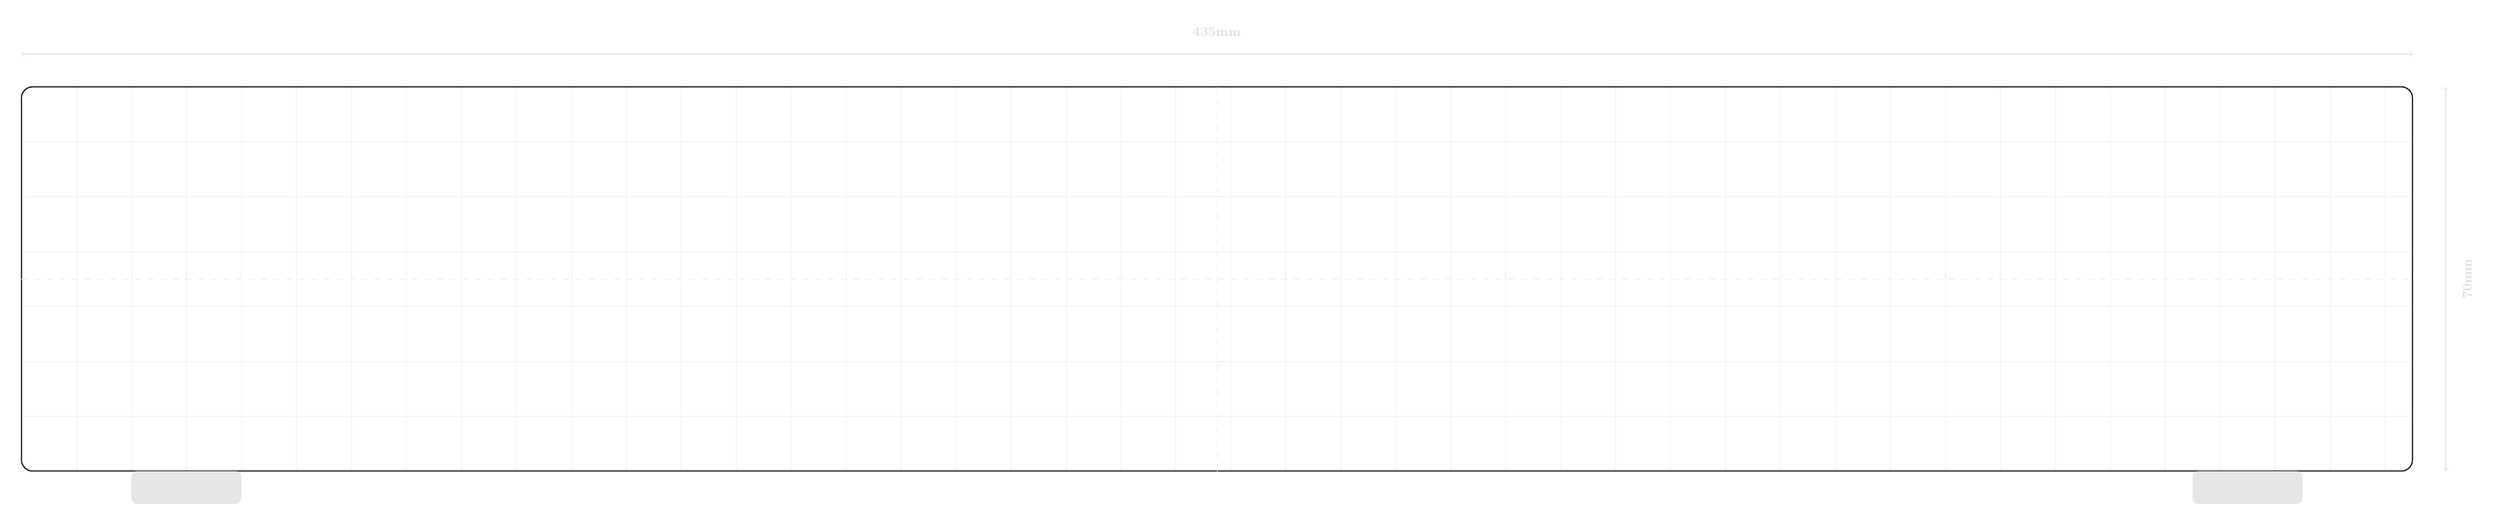
\begin{tikzpicture}[x=0.92mm, y=0.92mm]
  \def\cw{435} \def\ch{70}
  \begin{scope}
    \clip[rounded corners=1.8mm] (0,0) rectangle (\cw,\ch);
    \foreach \x in {0,10,...,435} { \draw[gray!12, line width=0.15pt] (\x,0) -- (\x,\ch); }
    \foreach \y in {0,10,...,70} { \draw[gray!12, line width=0.15pt] (0,\y) -- (\cw,\y); }
  \end{scope}
  \draw[black, line width=0.5pt, rounded corners=1.8mm] (0,0) rectangle (\cw,\ch);
  \draw[gray!15, line width=0.3pt, dashed] (\cw/2,0) -- (\cw/2,\ch);
  \draw[gray!15, line width=0.3pt, dashed] (0,\ch/2) -- (\cw,\ch/2);
  \fill[gray!20, rounded corners=1mm] (20,-6) rectangle (40,0);
  \fill[gray!20, rounded corners=1mm] (\cw-40,-6) rectangle (\cw-20,0);
  \draw[gray!30, line width=0.2pt, <->] (0,\ch+6) -- (\cw,\ch+6);
  \node[font=\fontsize{6}{8}\selectfont, text=gray!35] at (\cw/2,\ch+10) {435mm};
  \draw[gray!30, line width=0.2pt, <->] (\cw+6,0) -- (\cw+6,\ch);
  \node[font=\fontsize{6}{8}\selectfont, text=gray!35, rotate=90] at (\cw+10,\ch/2) {70mm};
\end{tikzpicture}
\end{center}

\newpage

%% ============================================================
%% PAGE 2: 435 x 102mm blank wireframe (92% scale)
%% ============================================================

\noindent
\begin{center}
{\fontsize{13}{16}\selectfont\bfseries TheStreamDeck -- Blank Wireframe (102mm)}\\[1pt]
{\fontsize{8}{10}\selectfont\color{gray} 92\% scale on A3 (actual: 435 x 102mm). Clean real estate for free sketching.}
\end{center}
\vspace{8mm}

\begin{center}
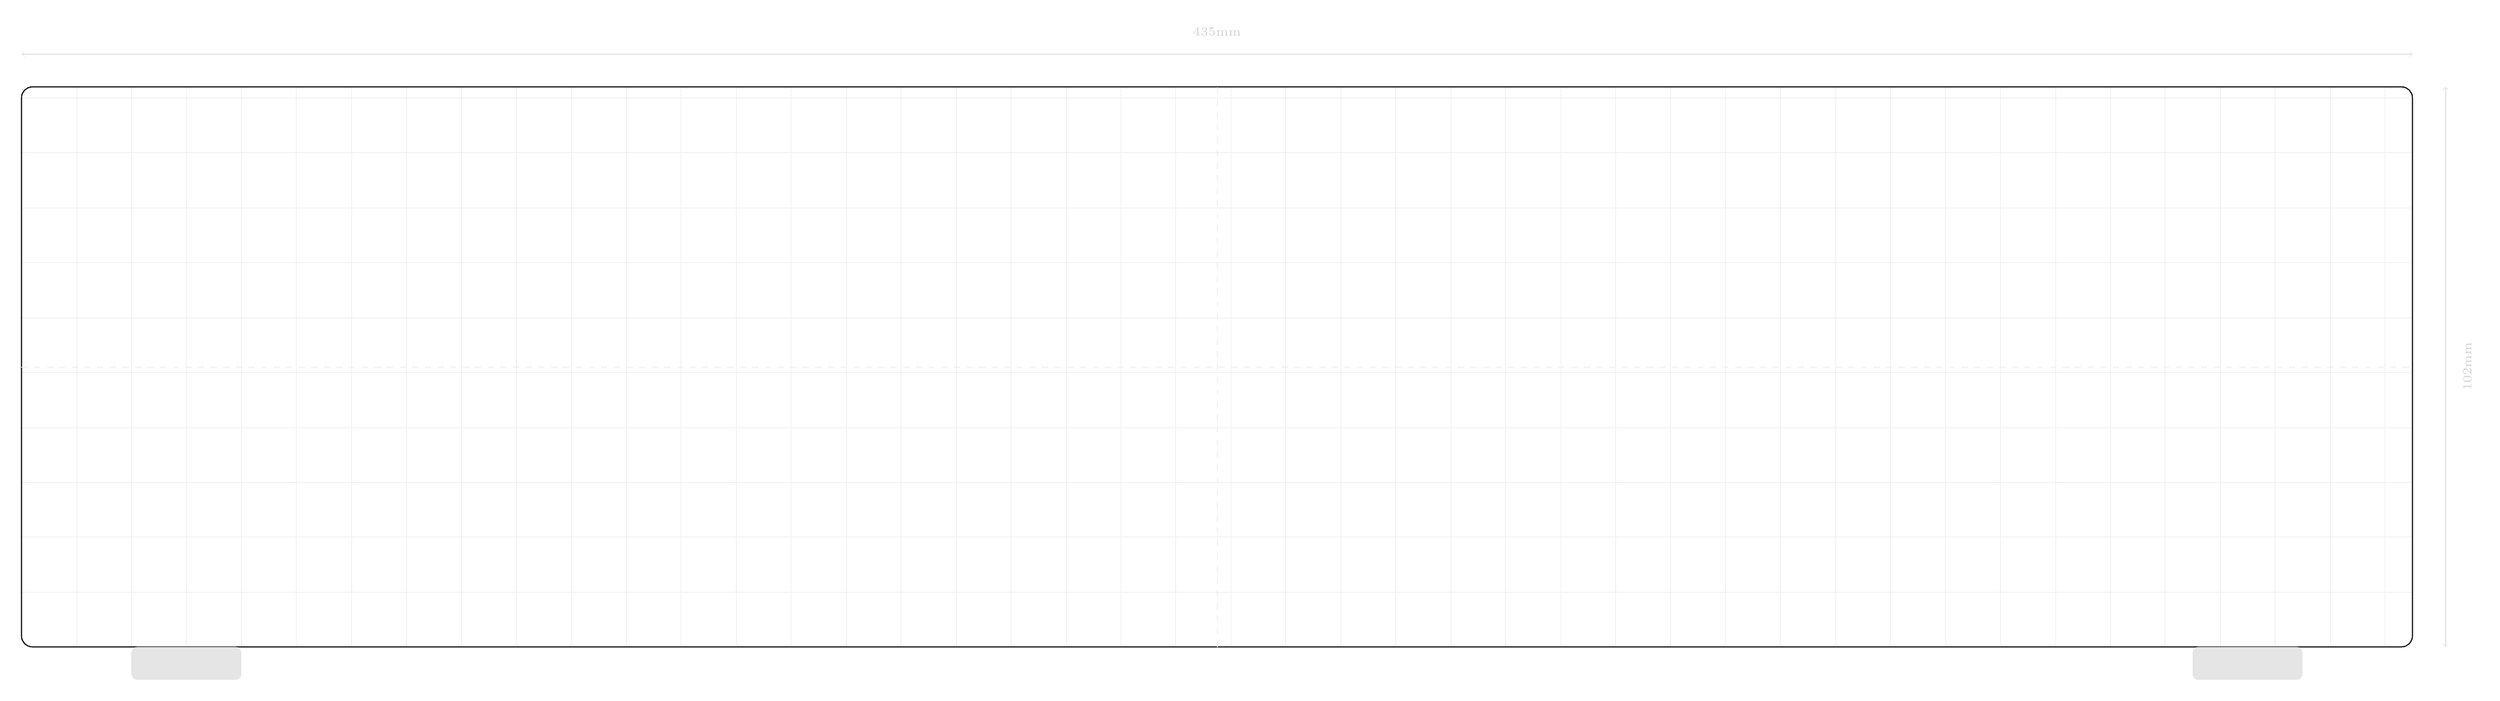
\begin{tikzpicture}[x=0.92mm, y=0.92mm]
  \def\cw{435} \def\ch{102}
  \begin{scope}
    \clip[rounded corners=1.8mm] (0,0) rectangle (\cw,\ch);
    \foreach \x in {0,10,...,435} { \draw[gray!12, line width=0.15pt] (\x,0) -- (\x,\ch); }
    \foreach \y in {0,10,...,110} { \draw[gray!12, line width=0.15pt] (0,\y) -- (\cw,\y); }
  \end{scope}
  \draw[black, line width=0.5pt, rounded corners=1.8mm] (0,0) rectangle (\cw,\ch);
  \draw[gray!15, line width=0.3pt, dashed] (\cw/2,0) -- (\cw/2,\ch);
  \draw[gray!15, line width=0.3pt, dashed] (0,\ch/2) -- (\cw,\ch/2);
  \fill[gray!20, rounded corners=1mm] (20,-6) rectangle (40,0);
  \fill[gray!20, rounded corners=1mm] (\cw-40,-6) rectangle (\cw-20,0);
  \draw[gray!30, line width=0.2pt, <->] (0,\ch+6) -- (\cw,\ch+6);
  \node[font=\fontsize{6}{8}\selectfont, text=gray!35] at (\cw/2,\ch+10) {435mm};
  \draw[gray!30, line width=0.2pt, <->] (\cw+6,0) -- (\cw+6,\ch);
  \node[font=\fontsize{6}{8}\selectfont, text=gray!35, rotate=90] at (\cw+10,\ch/2) {102mm};
\end{tikzpicture}
\end{center}

\vspace{12mm}

% Second copy
\begin{center}
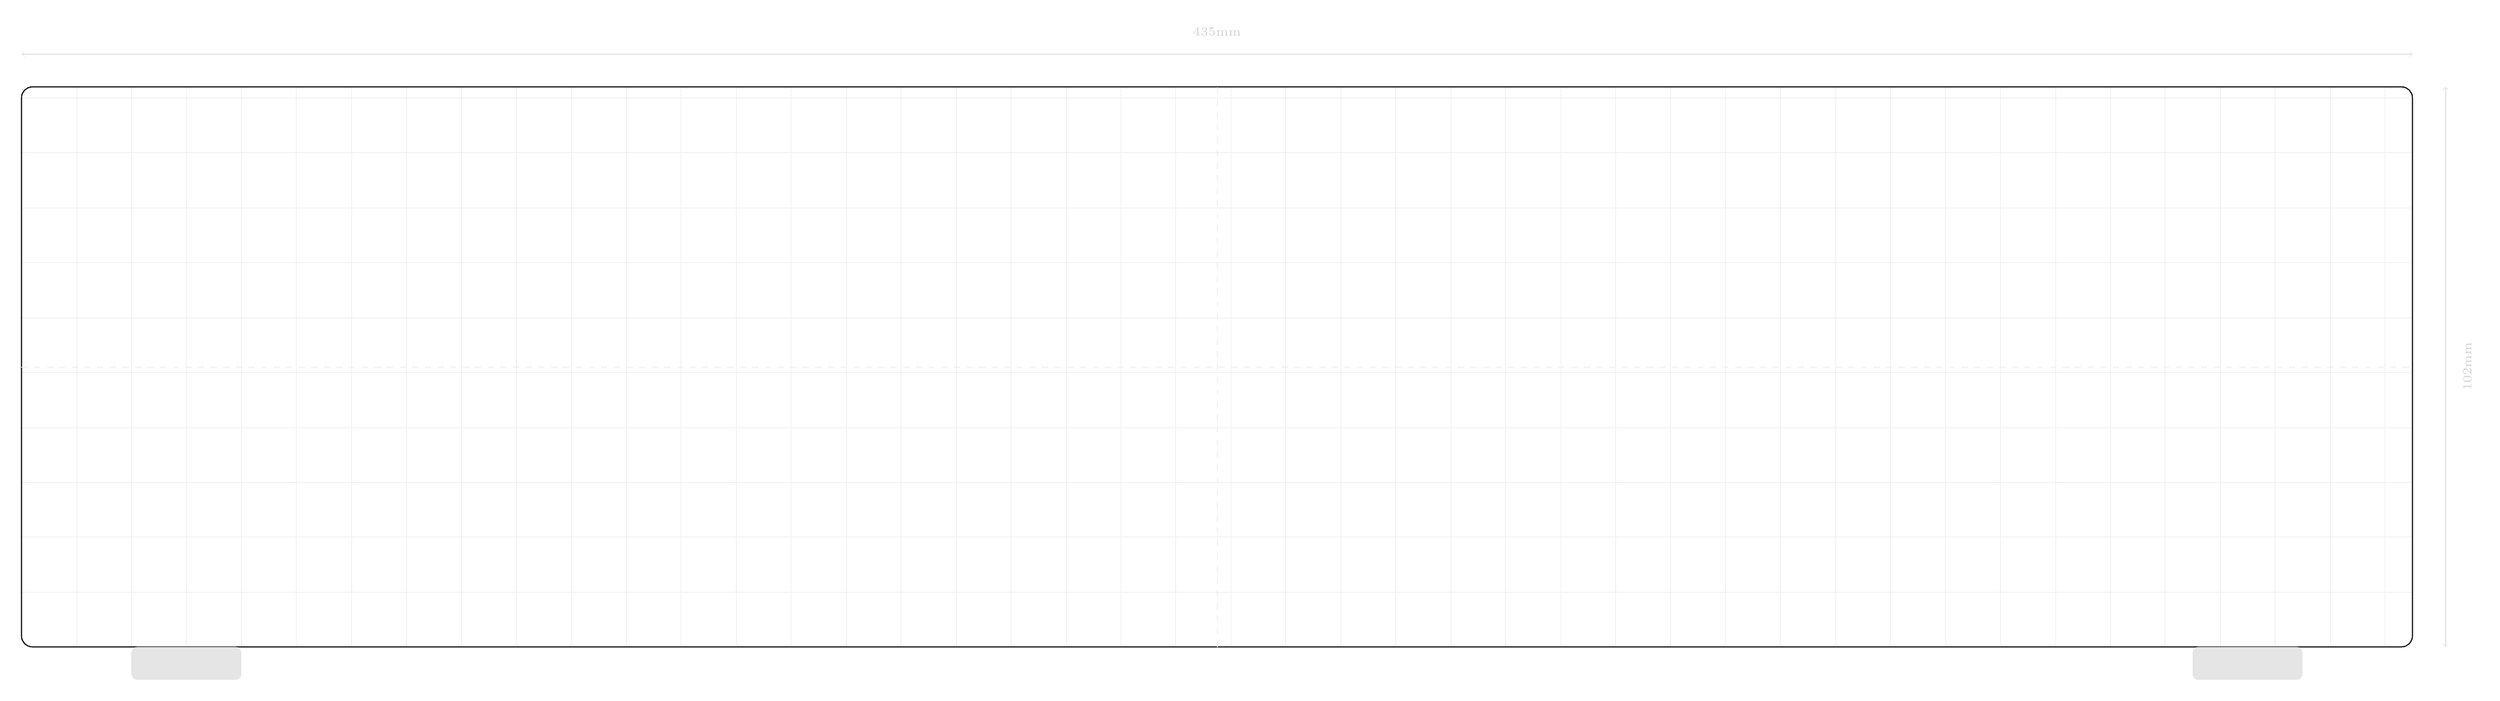
\begin{tikzpicture}[x=0.92mm, y=0.92mm]
  \def\cw{435} \def\ch{102}
  \begin{scope}
    \clip[rounded corners=1.8mm] (0,0) rectangle (\cw,\ch);
    \foreach \x in {0,10,...,435} { \draw[gray!12, line width=0.15pt] (\x,0) -- (\x,\ch); }
    \foreach \y in {0,10,...,110} { \draw[gray!12, line width=0.15pt] (0,\y) -- (\cw,\y); }
  \end{scope}
  \draw[black, line width=0.5pt, rounded corners=1.8mm] (0,0) rectangle (\cw,\ch);
  \draw[gray!15, line width=0.3pt, dashed] (\cw/2,0) -- (\cw/2,\ch);
  \draw[gray!15, line width=0.3pt, dashed] (0,\ch/2) -- (\cw,\ch/2);
  \fill[gray!20, rounded corners=1mm] (20,-6) rectangle (40,0);
  \fill[gray!20, rounded corners=1mm] (\cw-40,-6) rectangle (\cw-20,0);
  \draw[gray!30, line width=0.2pt, <->] (0,\ch+6) -- (\cw,\ch+6);
  \node[font=\fontsize{6}{8}\selectfont, text=gray!35] at (\cw/2,\ch+10) {435mm};
  \draw[gray!30, line width=0.2pt, <->] (\cw+6,0) -- (\cw+6,\ch);
  \node[font=\fontsize{6}{8}\selectfont, text=gray!35, rotate=90] at (\cw+10,\ch/2) {102mm};
\end{tikzpicture}
\end{center}

\end{document}
